\documentclass[convert={density=300,size=1080x800,outext=.png}]{standalone}

\usepackage[latin1]{inputenc}
\usepackage{tikz}

\usetikzlibrary{shapes,arrows,calc,fit,positioning}

\begin{document}
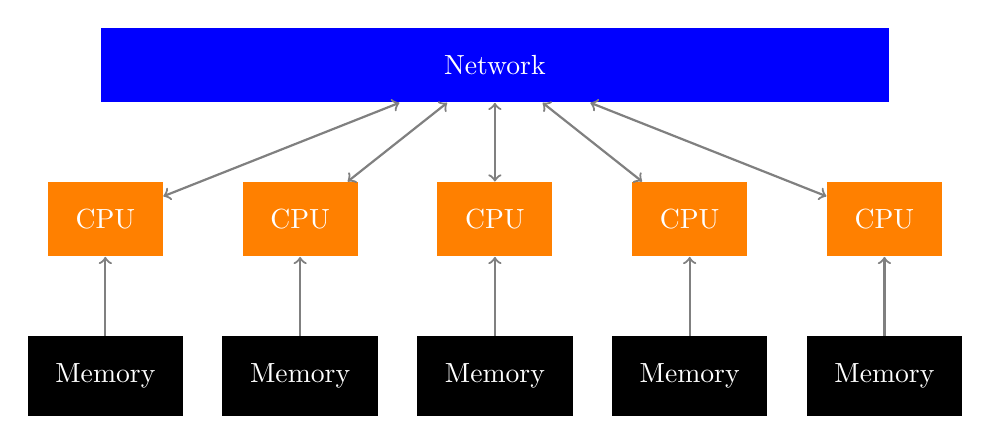
\begin{tikzpicture}[
  outer/.style={inner sep=10pt, text = white},
  block/.style={rectangle, draw, fill=blue!20}
  ]
  \node[outer, fill = blue, minimum width = 10cm] (A) { Network };
  \node[outer, fill = orange, below=of A] (B) { CPU };
  \node[outer, fill = orange, right=of B] (E) { CPU };
  \node[outer, fill = orange, right=of E] (F) { CPU };
  \node[outer, fill = orange, left=of B] (C) { CPU };
  \node[outer, fill = orange, left=of C] (D) { CPU };
  
  \node[outer, fill = black, below=of B] (G) { Memory };
  \node[outer, fill = black, below=of E] (H) { Memory };

  \node[outer, fill = black, below=of F] (I) { Memory };

  \node[outer, fill = black, below=of C] (J) { Memory };

  \node[outer, fill = black, below=of D] (K) { Memory };
  
  
  \draw[thick,black!50,<->] (B) -- (A);

  \draw[thick,black!50,<->] (D) -- (A);
  \draw[thick,black!50,<->] (C) -- (A);

  \draw[thick,black!50,<->] (E) -- (A);
  \draw[thick,black!50,<->] (F) -- (A);

  \draw[thick,black!50,->] (G) -- (B);

  \draw[thick,black!50,->] (H) -- (E);
  \draw[thick,black!50,->] (I) -- (F);

  \draw[thick,black!50,->] (J) -- (C);
  \draw[thick,black!50,->] (K) -- (D);
\end{tikzpicture}

\end{document}